\documentclass[10pt, compress]{beamer}  
\usetheme{metropolis}
%\usepackage{setspace} %this broke footnotes
\usepackage{epstopdf,amsmath,amsfonts,amssymb,amsthm}
\usepackage{jf}
\usepackage{hyperref}
%\usepackage[margin=1.0in]{geometry}
%\usepackage{placeins}
\usepackage{rotating}
%\usepackage[utf8]{inputenc}
\usepackage{booktabs}
\usepackage{pifont}
%\usepackage{tikz}
\usepackage{pgfplots}
\usepgfplotslibrary{dateplot}
\usepackage{tikzscale}
\usepgfplotslibrary{fillbetween}
%\usepackage[flushleft]{threeparttable}

\usepackage[most]{tcolorbox}% http://ctan.org/pkg/tcolorbox           
\usepackage[normalem]{ulem}                
\usepackage[scale=2]{ccicons}                 
\usepackage[super]{nth}                 
\usepackage{lmodern}
\newcommand{\semitransp}[2][35]{\color{fg!#1}#2}

%\usepackage{natbib}
%\bibliographystyle{jf}  
\usepackage[natbib, authordate, strict, backend=bibtex8, doi=only]{biblatex-chicago}
\addbibresource{sub/capacitybib.bib}
\usepackage{graphicx}
\usepackage[labelfont=bf,labelsep=period]{caption}   % Format figure 
\captionsetup[table]{labelsep=none}

\graphicspath{{.}{./sub/fig}}

%%%%%%%%Uncomment if making printable version for standout correction%%%%%%%
%\setbeamercolor{palette primary}{fg=black, bg=white}

\renewcommand\textbullet{\ensuremath{\bullet}}                  
\setbeamertemplate{bibliography item}{}           


\newcommand{\ctabtitle}[1]{\caption[#1]{\\ \textbf{#1}}}
\newcommand{\ctabsubtitle}[1]{\caption[#1]{\; \textit{#1}}}
\newcommand{\ctabnote}[1]{\begin{flushleft} #1 \end{flushleft}}

\newcommand{\cfigcaption}[2]{\caption[#1]{\textbf{\\#1} \\ #2}}
\newcommand{\cfigtitle}[1]{\caption[#1]{ \\ \textbf{#1} }}
\newcommand{\cfigbeamcaption}[1]{\caption*{\\ #1}}

%Chernov Method
%1) What is the problem?
%2) WHy is it important?
%3) How are you solving the problem?
%4) Results

%%%%%%%%%%%%%Kicker boxes
\definecolor{zaffre}{rgb}{0.0, 0.08, 0.66}
\newtcolorbox{kicker}{colback=zaffre,arc=0.5mm,coltext=white, fontupper=\bfseries, colframe=black, halign=flush left, left=0.75mm, top=0.75mm, bottom=0.75mm, right=0.75mm}

\definecolor{mgrey}{rgb}{0.2824,0.3176,0.298}
\definecolor{lgrey}{rgb}{.7176, .7451, .7333}
\definecolor{vlgrey}{rgb}{.9098, .9176, .9137}
\newtcolorbox{quotebox}[1]{colback=vlgrey,
colframe=mgrey,fonttitle=\bfseries,
title=#1, left=1mm, top=1mm, bottom=1mm, right=1mm}
%%%%%%%%%%%%%%%%%%%%%%%
%Variable fonts per slide
%https://tex.stackexchange.com/questions/33969/changing-font-size-of-selected-slides-in-beamer
\usepackage{environ}
\usepackage{lipsum}

%
% Custom font for a frame.
%
\newcommand{\customframefont}[1]{
\setbeamertemplate{itemize/enumerate body begin}{#1}
\setbeamertemplate{itemize/enumerate subbody begin}{#1}
}

\NewEnviron{framefont}[1]{
\customframefont{#1} % for itemize/enumerate
{#1 % For the text outside itemize/enumerate
\BODY
}
\customframefont{\normalsize}
}

\setbeamercolor{background canvas}{bg=white}
%%%%%%%%%%%%%%%%%%%%%%%%%%%%%


%Some stuff from a previous document, not totallly sure what this is
\setbeamertemplate{blocks}[rounded][shadow=true]                  
\metroset{block=fill}                 
\definecolor{mycolor}{rgb}{0.122, 0.435, 0.698}% Rule colour
\makeatletter


\makeatother
%\author[Tepper]{Clinton Tepper\inst{\text{\ding{169}}}}
%\institute[]{\inst{\text{\ding{169}}} UCLA Anderson School of Management}
\author[Tepper]{iCapital Portfolio Analytics}
\title{\Large \bf GMAM 3.0: Preqin Data}

\date{\today}

\begin{document}

\newcommand{\tstar}{\ensuremath{^\text{***}}}
\newcommand{\dstar}{\ensuremath{^\text{**}}}
\newcommand{\ostar}{\ensuremath{^\text{*}}}
\maketitle

%%%%%%%%%%%%%%%%%%%%%%%%%%%%%%%%%%%


%\begin{frame}[fragile]
%\frametitle{The Research Process}
%\begin{figure}
%	\centering
%	%\includegraphics[width=0.95\linewidth]{sub/fig/paxsectionalverification-mfs.pdf}
	%\includegraphics[width=0.95\linewidth]{sub/fig/xmomassetsfs.tikz}
%	\includegraphics[width=1.04\linewidth]{docs/theory/Model Development.pdf}\\
%    \bigskip
%\end{figure}

%\end{frame}

\begin{frame}[fragile]
\frametitle{Preqin Data} \label{fr:motivation}
\begin{itemize}
    \item Cashflow-only metrics are biased because at each point in time, only the managers with the best performance will realize returns.
    \item []
    \item For many asset allocation decisions, time-weighted returns based on market value are of particular interest.
    \item []
    \item Preqin data provides the necessary information for computing time-weighted returns on private equity investments.
\end{itemize}
\end{frame}

\begin{frame}[fragile]
\frametitle{Time-weighted Returns} \label{fr:motivation}
\begin{itemize}
    \item  While not the traditional way of looking at private capital. 
    \item []
    \item Yet it is necessary to analyze the risk characteristics of a portfolio conditional on current allocations, as well as asset class performance.
    \item []
    \item It is also important for many types of allocation decisions.
    \begin{itemize}
        \item For example, consider a portfolio manager that holds a private equity investment making an allocation decision between stocks and bonds.
    \end{itemize}
    \item []
    \item The downside is it may deviate from the returns an investor realizes over the life of the fund.
    \item []
    \item Adjustments to the return calculations can mitigate some of the downside at the cost of accounting complexity, and warrant future discussion and research.
\end{itemize}
\end{frame}


\begin{frame}[fragile]
\frametitle{Preqin data: calculations} \label{fr:motivation}
\begin{itemize}
    \item  The standard return calculation:
    \begin{align*}
        R_t &= \frac{NAV_t + CF_t}{NAV_{t-1}}
    \end{align*}
    where $NAV$ is the fund's net asset value and $CF$ is the net cashflows.
    \item Compute $NAV$ from the capital paid in ($PI$) and the residual value ratio ($RVPI$):
    \begin{align*}
        NAV_t &= PI_t\times RVPI_t\\
        PI_t &= CC_t\% \times \text{[Total Committed Capital]}
    \end{align*}
    \item []
    \item Compute cashflows from the capital committment ratio and distribution ratio
    \begin{align*}
        CF_t &= DPI_t\times PI_t - DPI_{t-1} \times PI_{t-1}- \left(PI_t-PI_{t-1}\right)
    \end{align*}
\end{itemize}
\end{frame}

\begin{frame}[fragile]
\frametitle{Complications} \label{fr:motivation}
\begin{itemize}
    \item Preqin does not provide  total capital committed, so substitute a dummy value (this will not affect the returns)
    \item []
    \item Performance realized during periods of low NAV is a poor measure of investment performance
    \begin{itemize}
        \item Ignore holdback performance and performance where only a small percentage of capital is called.
        \item Mitigates some of the downside of time-weighted returns.
    \end{itemize}
    \item []
    \item Missing data
\end{itemize}
\end{frame}


\begin{frame}[fragile]
\frametitle{Preliminary performance} \label{fr:motivation}
\begin{itemize}
    \item Assign a prior that investment in a private equity fund is the same as an investment in the public market factor.
    \item []
    \item Prior is weakly informative.
    \item []
    \item Continue MCMC simulation until an equivalent sample size of 20 independent draws is realized, as measured using a systematically tuned non-parametric moving block bootstrap.
\end{itemize}
\end{frame}


\begin{frame}[fragile]

\begin{figure}
	\centering
	%\includegraphics[width=0.95\linewidth]{sub/fig/paxsectionalverification-mfs.pdf}
	%\includegraphics[width=0.95\linewidth]{sub/fig/xmomassetsfs.tikz}
	\includegraphics[width=1.04\linewidth]{docs/fig/Abbott.pdf}\\
    \bigskip

\end{figure}
\end{frame}

\begin{frame}[fragile]

\begin{figure}
	\centering
	%\includegraphics[width=0.95\linewidth]{sub/fig/paxsectionalverification-mfs.pdf}
	%\includegraphics[width=0.95\linewidth]{sub/fig/xmomassetsfs.tikz}
	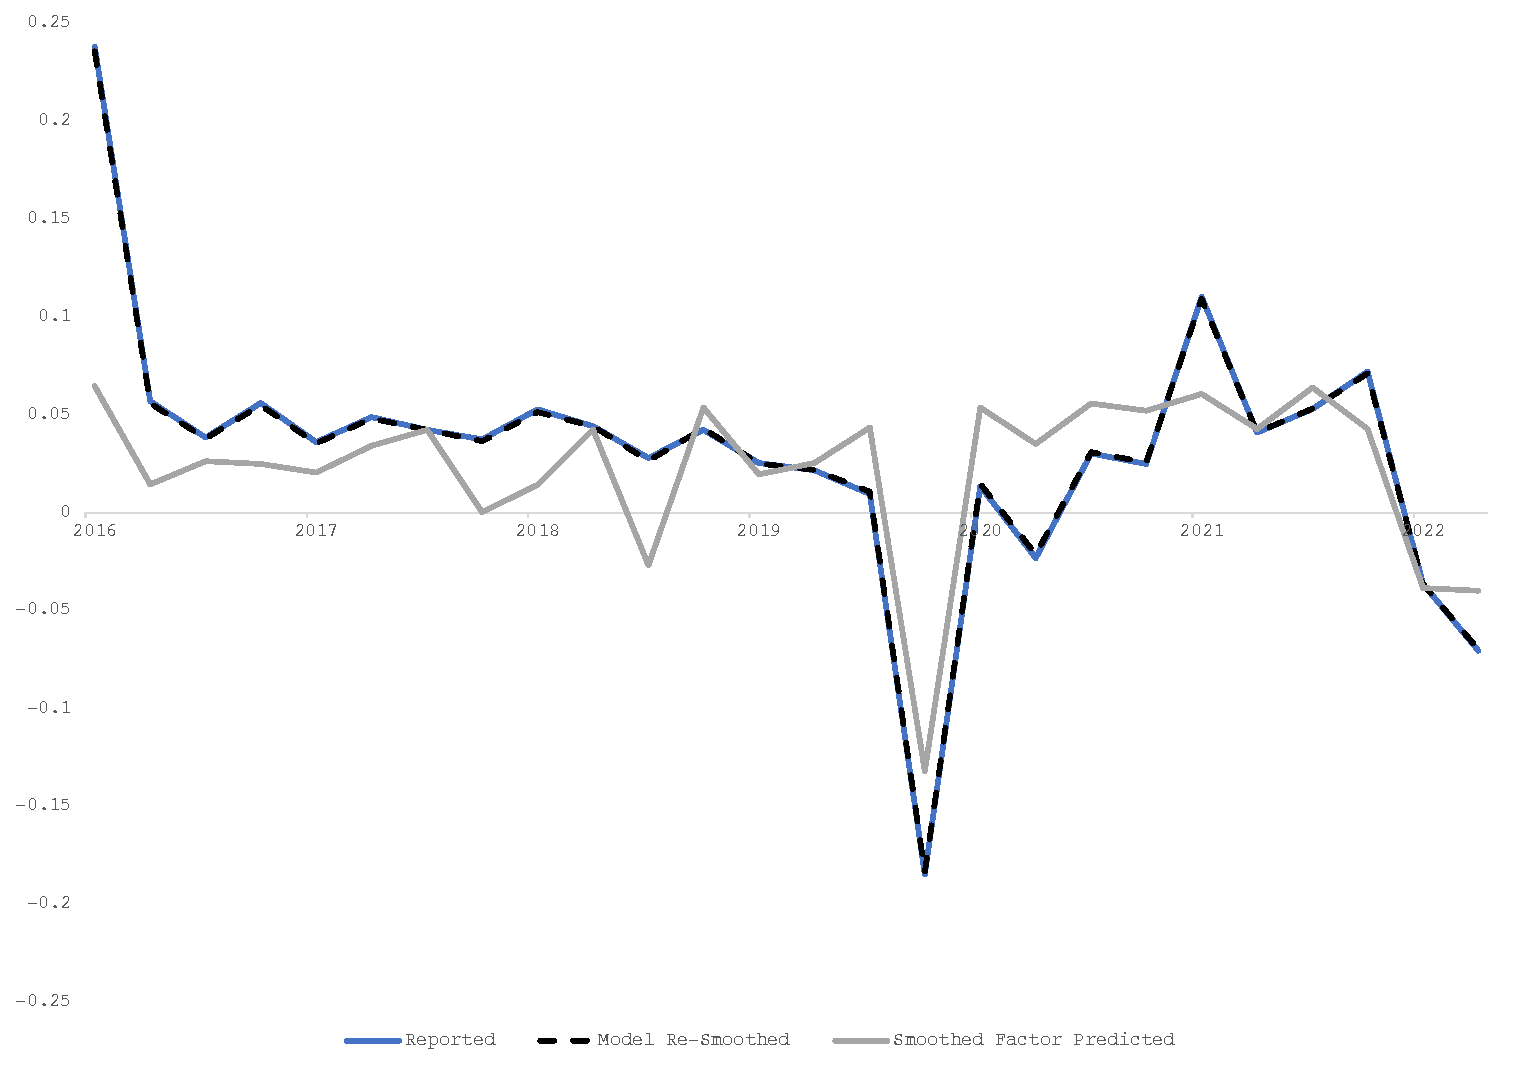
\includegraphics[width=1.04\linewidth]{docs/fig/RockpointV.pdf}\\
    \bigskip

\end{figure}
\end{frame}


\begin{frame}[fragile]

\begin{figure}
	\centering
	%\includegraphics[width=0.95\linewidth]{sub/fig/paxsectionalverification-mfs.pdf}
	%\includegraphics[width=0.95\linewidth]{sub/fig/xmomassetsfs.tikz}
	\includegraphics[width=1.04\linewidth]{docs/fig/Freeman.pdf}\\
    \bigskip

\end{figure}

\end{frame}





\end{document}